\chapter{From Analog to Digital}

Our everyday experience of sound is an entirely analog one. When a physical     object emits or reflects a sound wave into space and towards our ears, the signal produced consists of an infinite set of values, spaced apart in infinitesimal intervals. Due to the fact that such a signal has an amplitude value at every single point in time, it is called a continuous signal. \citedsp{11} Figure \ref{fig:cont} displays the continuous representation of a sine wave.

\begin{figure}[h!]

  \centering

  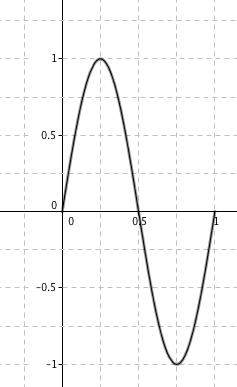
\includegraphics[scale=0.5]{img/cont}

  \caption{The continuous representation of a typical sine wave. In this case, both the signal's frequency $f$ as well as the maximum elongation from the equilibrium $a$ are equal to $1$. }

  \label{fig:cont}

\end{figure}

\pagebreak

\noindent While continuous signals and the idea of an infinite, uncountable set of values are easy to model in mathematics and physics --- the analog world, computers --- in the digital world --- effectively have no means by which to represent something that is infinite, since computer memory is a finite resource. Therefore, signals in the digital domain are discrete, meaning they are composed of periodic \emph{samples}. A sample is a discrete recording of a continuous signal's amplitude, taken in a constant time interval. The process by which a continuous signal is converted to a discrete signal is called \emph{quantization}, \emph{digitization} or simply \emph{analog-to-digital-conversion} \citedsp{35-36}. Quantization essentially converts an analog function of amplitude to a digital function of location in computer memory over time (Burk, Polansky, Repetto, Roberts and Rockmore, 2011, Section 2.1). The reverse process of converting discrete samples to a continuous signal is called \emph{digital-to-analog-conversion}. Figure \ref{fig:disc} shows the discrete representation of a sine wave, the same signal that was previously shown as a continuous signal in Figure \ref{fig:cont}. \citebs{16-17}

\begin{figure}[h!]

  \centering

  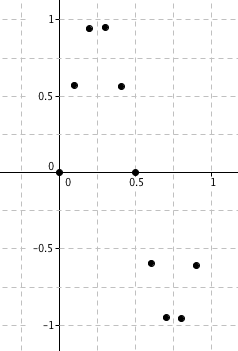
\includegraphics[scale=0.5]{img/disc}

  \caption{The discrete representation of a typical sine wave.}

  \label{fig:disc}

\end{figure}

\section{Sample Rate}

The sample rate (often referred to as sampling rate or sampling frequency), commonly denoted by $f_{s}$, is the rate at which samples of a continuous signal are taken to quantize it. The value of the sample rate is measured in Hertz (Hz) or samples per second. Common values for audio sampling rates are 44.1 kHz, a frequency originally chosen by Sony in 1979 that is still used for Compact Discs, and 48 kHz, the standard audio sampling rate used today. \citebs{18} (Colletti, 2013) The reciprocal of the sample rate yields the sampling interval, denoted by $T_{s}$ and measured in seconds, which is the time period after which a single sample is taken from a continuous signal:

\begin{equation}
   T_{s} = \frac{1}{f_{s}}
\end{equation}

\noindent The reciprocal of the sample interval again yields the sampling rate:

\begin{equation}
  f_{s} = \frac{1}{T_{s}}
\end{equation}

\section{Nyquist Limit}

The sample rate also determines the range of frequencies that can be represented by a digital sound system. The reason for this is that only frequencies that are less than or equal to one half of the sampling rate can be "properly sampled". To sample a signal "properly" means to be able to reconstruct a continuous signal, given a set of discrete samples, exactly, i.e. without any \emph{quantization errors}. This is only possible if the frequency of a signal allows at least one sample per cycle to be taken above the equilibrium and at least one sample below. The value of one half of the sample rate is called the \emph{Nyquist frequency} or \emph{Nyquist limit}, named after Harry Nyquist, who first described the Nyquist limit and associated phenomena together with Claude Shannon in the 1940s, stating that "a continuous signal can be properly sampled, only if it does not contain frequency components above one half the sampling rate". Any frequencies above the Nyquist limit lead to \emph{aliasing}, which is discussed in the next section. \citedsp{40}

Given the definition of the Nyquist limit and considering the fact that the limit of human hearing is approximately 20 kHz (Cutnell \& Johnson, 1998, p. 466), the reason for which the two most common audio sample rates are 40 kHz and above is clear: they were chosen to allow the "proper" representation of the entire range of frequencies audible to humans, since a sample rate of 40 kHz or higher meets the Nyquist requirement of a sample rate at least twice the maximum frequency component of the signal to be sampled (the Nyquist limit), in this case ca. 20 Khz.

\section{Aliasing}

When a signal's frequency exceeds the Nyquist limit, it is said to produce an \emph{alias}, a new signal with a different frequency that is indistinguishable from the original signal when sampled. This is due to the fact that a signal with a frequency component above the Nyquist limit no longer has one sample taken above and one below the zero level for each cycle, but at arbitrary points of the original signal. When these points are connected, they yield an entirely different signal. For example, if the sinusoid depicted in Figure \ref{fig:orig}, with a frequency of 4 Hz, is sampled at a sample rate of 5 Hertz, shown in Figure \ref{fig:sampled}, meaning the frequency of the continuous signal is higher than the Nyquist limit (here 2.5 Hz), the reconstructed signal, approximated in Figure \ref{fig:approx}, will look completely different from the original sinusoid. "This phenomenon of [signals] changing frequency during sampling is called aliasing, [...] an example of improper sampling". \citedsp{40}

\begin{figure}[p!]

  \centering

  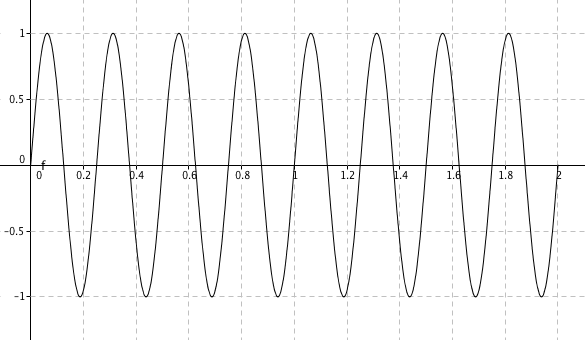
\includegraphics[scale=0.5]{img/orig}

  \caption{A sinusoid with a frequency of 4 Hz.}

  \label{fig:orig}

\end{figure}

\begin{figure}[p!]

  \centering

  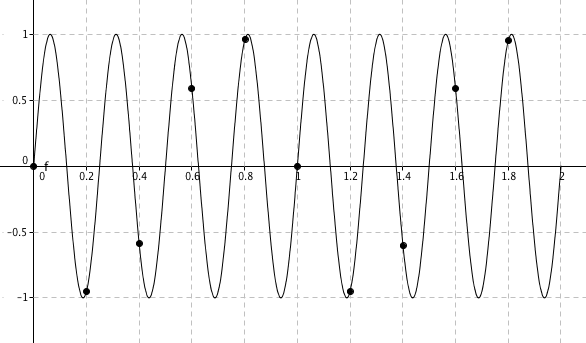
\includegraphics[scale=0.5]{img/sampled}

  \caption{A sinusoid with a frequency of 4 Hz, sampled at a sample rate of 5 Hz. According to the Nyquist Theorem, this signal is sampled improperly, as the frequency of the continuous signal is not less than or equal to one half of the sample rate, in this case 2.5 Hz. }

  \label{fig:sampled}

\end{figure}

\begin{figure}[p!]

  \centering

  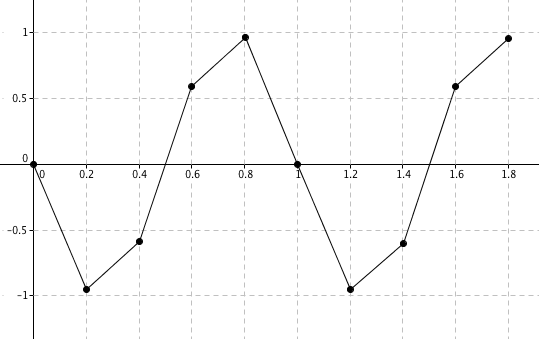
\includegraphics[scale=0.5]{img/approx}

  \caption{An approximated representation of the signal created from the sampling process shown in Figure \ref{fig:sampled}. Visually as well as acoustically, the new signal is completely different from the original signal. However, in terms of sampling, they are indistinguishable from each other due to improper sampling. These signals are said to be \emph{aliases} of each other.}

  \label{fig:approx}

\end{figure}

\pagebreak

\section{Overflow}

Another interesting property of digital sound, which is not encountered in the analog realm, is that it can overflow. If one attempts to increase the loudness of something in the analog world, for example by hitting a drum more intensely, the expected result is a louder sound. In the digital realm however, it may occur that attempting to increase a signal's amplitude does not result in an increased loudness, but in distortion. The cause of this phenomenon lies in the way digital audio is stored. Since computer memory is a finite resource, each sample has a dedicated portion of computer memory allocated to it. For example, the Waveform Audio File Format (WAVE), a common computer file format for audio data, stores each sample of an audio track as a 16-bit signed integer. A 16-bit signed integer gives a possible range of $-2^{16-1}$ to $2^{16-1}$ ($16-1$ because the most significant bit is used as the sign bit in two's complement representation). This means that a signal with an amplitude of 1 will be stored as 32767, an amplitude of 0.5 as 16384, an amplitude of -1 as -32768 and so on. If one tries to increase the amplitude of a signal whose value has already saturated the available range and space allocated to it, in this case 32767 on the positive end and -32768 on the negative end, the result is that the integer with which the sample is stored \emph{overflows}. Because WAVE files (and many other storage media) store samples as \emph{signed} integers, overflow always results in a change of sign:

$$32767_{10} = 0111111111111111_{2}$$
$$0111111111111111_{2} + 1 = 1000000000000000_{2} = -32768_{10}$$
$$1000000000000000_{2} - 1 = 0111111111111111_{2} = 32767_{10}$$

A visualization of the result of increasing the amplitude of a signal with a saturated value (an amplitude of 1), shown in Figure \ref{fig:no-over}, is given in Figure \ref{fig:over}.

\begin{figure}[h!]

  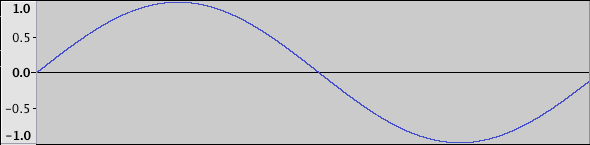
\includegraphics[scale=0.5]{img/no-over}

  \caption{A typical sinusoidal signal with an amplitude of 1. The integer range provided by the allocated memory for the top-most sample is saturated, meaning it is equal to $32767_{10}$ or $0111111111111111_{2}$.}

  \label{fig:no-over}

\end{figure}

\begin{figure}[h!]

  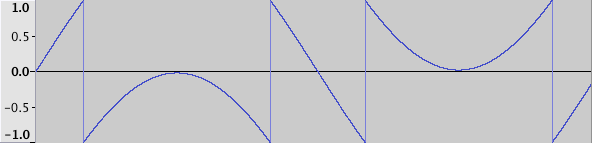
\includegraphics[scale=0.5]{img/over}

  \caption{What happens when the amplitude of the signal from Figure \ref{fig:no-over} is increased by a factor of 2. Multiple samples have overflowed and thus changed their sign. Because of the way two's-complement representation is implemented, the signal continues it's path as if no overflow had ever occurred. The only difference being that the sign has changed mid-way.}

  \label{fig:over}

\end{figure}
